Die Hauptaufgabe einer modernen Universitätsbibliothek ist es,
ihre Nutzer*innen zu unterstützen.
Dies geschieht vor allem dadurch,
dass Informationen zugänglich gemacht werden.
Früher wurde dies durch Zettelkataloge,
in denen die Bücher verzeichnet waren,
erreicht.
Im Rahmen der Formal\babelhyphen{soft}erschließung
wurden hier Informationen,
wie zum Beispiel der Titel, der Autor und die \gls{isbn} dokumentiert.
Für die Sach\babelhyphen{soft}erschließung wurden diese formalen Informationen
um inhaltliche Informationen ergänzt.
Hierfür gab es dann nach Themen sortierte Zettelkästen,
wie in \Cref{fig:zettelkasten} zu sehen ist.
\begin{figure}
	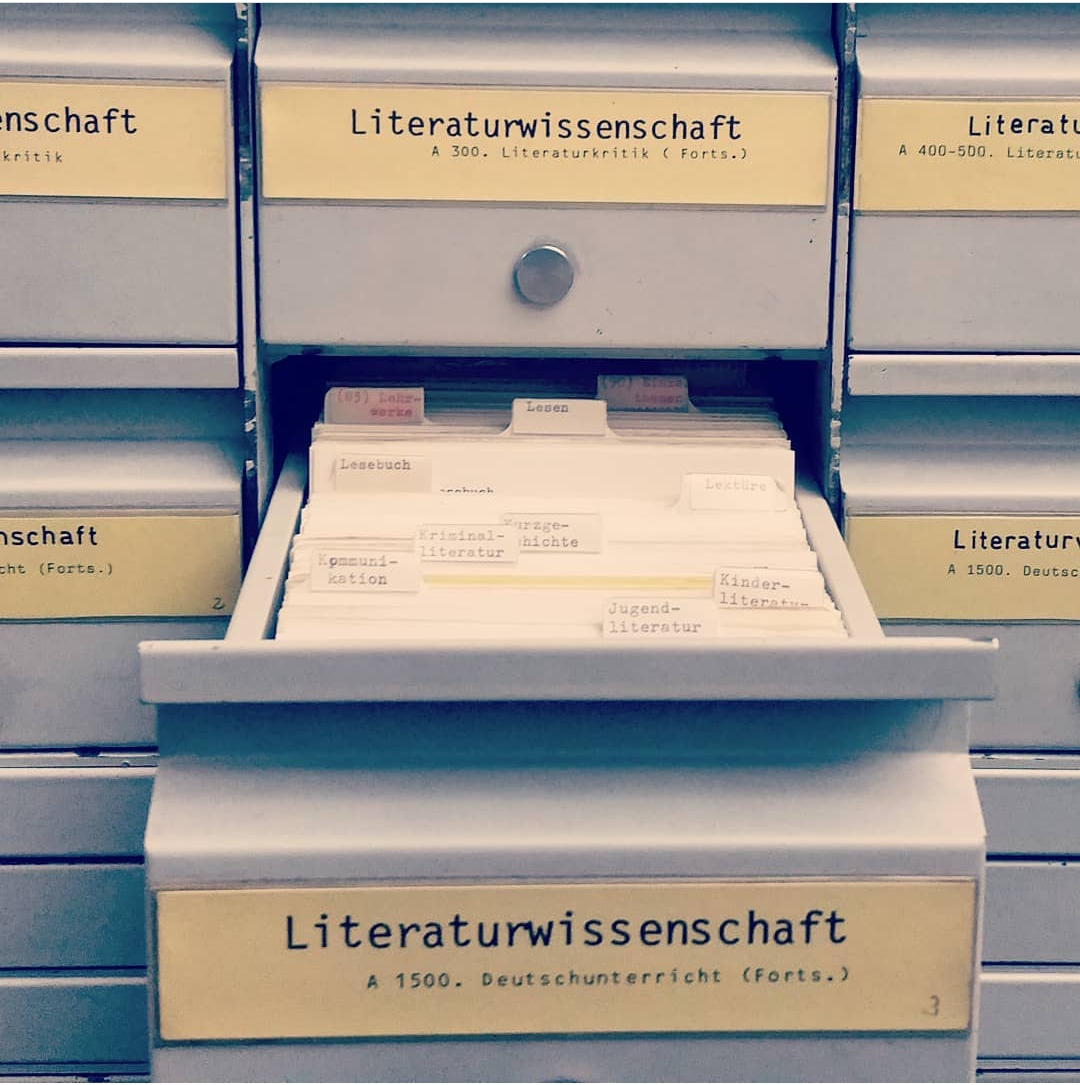
\includegraphics[keepaspectratio, width=\textwidth]{figures/Zettelkasten.jpg}
	\caption{Zettelkasten aus der \gls{jcs}. Quelle: {Petra Schneider}}
	\label{fig:zettelkasten}
\end{figure}
Die Zettelkästen wurden an der \gls{jcs},
wie auch an vielen anderen Bibliotheken,
durch einen \gls{opac} ersetzt,
der den Zugriff auf die Übersicht von überall bietet.
Als zusätzlicher Vorteil kommt bei digitalen Lösungen
die einfachere Suche über verschiedene Felder eines Eintrags hinzu.

Eine manuelle Sacherschließung hängt von den Fähigkeiten der erfassenden Person ab.
Somit ist,
trotz bibliothekarischer Regelwerke,
nicht sichergestellt,
dass alle relevanten Schlagworte und Themenkomplexe verzeichnet werden.
Die vollständige Verschlagwortung und Verknüpfung mit zusätzlichem Wissen
ist der Schritt Richtung \enquote{Semantic Web}
und Zukunft der Bibliotheken.
Durch solche Verknüpfungen wird die Information für die Nutzer noch besser zugänglich,
denn vom Eintrag sind die Themenbereiche zu erreichen,
welche auf alle Einträge verweisen.
Dies vereinfacht die Suche.

Im Rahmen dieser Aufgabe betreut die \gls{jcs}
mehrere \glspl{fachinformationsdienst}
mit finanzieller Förderung der \gls{dfg}
über deren Förderprogramm \enquote{Fachinformationsdienste für die Wissenschaft}
\footnote{\url{https://www.dfg.de/foerderung/programme/infrastruktur/lis/lis_foerderangebote/fachinfodienste_wissenschaft/index.html}}.
Diese sind in \cref{fig:fid:overview} dargestellt.

\begin{table}
	\begin{tabularx}{\textwidth}{l r}
		Afrikastudien                                      & \multirow{2}{*}{\href{http://www.ilissafrica.de/}{
\includegraphics[height=1cm]{figures/ilissLogo.png}}}            \\ \footnotesize{\url{http://www.ilissafrica.de/}} &\\[2ex]
		Allgemeine und Vergleichende Literaturwissenschaft & \multirow{2}{*}{\href{http://avldigital.de/}{
\includegraphics[height=1cm]{figures/avl.png}}}                       \\ \footnotesize{\url{http://avldigital.de/}}&\\[2ex]
		Biodiversitätsforschung                            & \multirow{2}{*}{\href{https://www.biofid.de/de/}{
\includegraphics[height=1cm]{figures/biofid_160.png}}}            \\ \footnotesize{\url{https://www.biofid.de/de/}} & \\[2ex]
		Darstellende Kunst                                 & \multirow{2}{*}{\href{http://www.performing-arts.eu/}{
\includegraphics[height=1cm]{figures/fid-dk_160.png}}}       \\ \footnotesize{\url{http://www.performing-arts.eu/}} & \\[2ex]
		Germanistik                                        & \multirow{2}{*}{\href{https://www.germanistik-im-netz.de/}{
\includegraphics[height=1cm]{figures/gin_logo150.png}}} \\ \footnotesize{\url{https://www.germanistik-im-netz.de/}} & \\[2ex]
		Jüdische Studien                                   & \multirow{2}{*}{\href{https://www.jewishstudies.de/}{
\includegraphics[height=1cm]{figures/fid-js_160.png}}}        \\ \footnotesize{\url{https://www.jewishstudies.de/}} & \\[2ex]
		Linguistik                                         & \multirow{2}{*}{\href{http://www.linguistik.de/}{
\includegraphics[height=1cm]{figures/linguistik_160.png}}}        \\ \footnotesize{\url{http://www.linguistik.de}} &
	\end{tabularx}
	\caption{Übersicht der \glspl{fachinformationsdienst} der \gls{jcs} \autocite{ub:sammlungen:fid}}
	\label{fig:fid:overview}
\end{table}

Der \gls{fachinformationsdienst} Linguistik ist
\textquote[\autocite{ub:projekte:fid-linguistik}]{ein Kooperationsprojekt zwischen der Universitätsbibliothek Johann Christian Senckenberg und  Prof. Christian Chiarcos vom Forschungsgebiet Angewandte Computerlinguistik (AcoLi) am Institut für Informatik der Goethe Universität}
und betreibt das Lin|gu|is|tik-Portal,
welches im folgenden Abschnitt beschrieben wird.

\subsection{Das Portal}
\blockquote[\autocite{ub:projekte:fid-linguistik}]{Das Lin|gu|is|tik-Portal ist
	ein Fachportal für die allgemeine und vergleichende Sprachwissenschaft
	sowie die Linguistiken der europäischen und außereuropäischen Einzelphilologien.}
Es weist
die Titelmetadaten,
wie z.B.\, den Autor, den Titel oder das Thema,
verschiedener Publikationen nach.
Um den Nutzen für die Forschung zu steigern,
soll in Zukunft eine Volltextsuche über die \gls{openaccess}[-Texte]
hinzugefügt werden.
Diese soll durch einen Index auf Basis von \glspl{knowledgebase},
wie z.B.\, der \gls{bllontology}, WikiData oder GND-Sachbegriffen
unterstützt werden,
indem die Volltexte mit semantischen Deskriptoren versehen werden.

\subsection{Die Ziele}
\label{ssec:ziele}
Das Ziel dieser Arbeit ist die Implementierung eines mehrschrittigen Prozesses.
Zuerst sollen \glsfirst{bll}[-Termini] in linguistischen Texten erkannt werden (\gls{namedentityrecognition}).
Diesen Schritt bezeichnet man teilweise als \gls{mentiondetection},
denn die meisten Prozesse erkennen hier noch keine Entitäten.
Stattdessen werden Kandidaten für Entitäten erkannt.
Nachdem diese Kandidaten erkannt sind,
werden im Schritt der \gls{namedentitydisambiguation}
die gefundenen Kandidaten mit der \gls{knowledgebase} abgeglichen.
Um diesen Abgleich effizienter zu machen,
wird oft für jede Mention eine Liste von möglichen Kanditation aus der \gls{knowledgebase} extrahiert
(English: \foreigntextquote{english}{Candidate Generation})\autocite{Raheim2022}
und der geeignetste Kanditat aus der \gls{knowledgebase} ausgewählt.
Dies ist insbesondere bei sehr breiten \glspl{knowledgebase} wichtig,
in denen Benennung von Entitäten mehrfach vorkommen;
so listet \citeauthor{dewiki:209960843}
für die Abkürzung \emph{FFM}\autocite{dewiki:209960843}
neben der Bedeutung \emph{Frankfurt am Main}\autocite{dewiki:225740004} noch 14 weitere Bedeutungen,
wie in \cref{tbl:ffm} zu sehen ist,
zwischen denen aus dem Kontext entschieden werden müsste.

\begin{table}
	\begin{tabularx}{\textwidth}{l l}
		Fachschule für Foto- und Medientechnik & Fixed Frequency Modem              \\
		Fast Food Musical                      & Frankfurt am Main                  \\
		Fédération française de motocyclisme   & Frankfurter Feldbahnmuseum         \\
		Fédération Française Motonautique      & Fudbalska Federacija na Makedonija \\
		Female Female Male                     & Fünf-Faktoren-Modell               \\
		Festival des Films du Monde            & Full Face Mask                     \\
		Fettfreie Masse                        & Fused Filament Fabrication         \\
		Firefly                                & Maasina-Fulfulde
	\end{tabularx}
	\caption{
		Übersicht der Bedeutungen der Abkürzung \emph{FFM}, bzw.\, \emph{ffm}
		nach \citetitle{dewiki:209960843} \autocite{dewiki:209960843}
	}
	\label{tbl:ffm}
\end{table}

Im letzten Schritt wird die Mention im Text mit dem ausgewählten Kanditaten aus der \gls{knowledgebase}
annotiert bzw.\, verknüpft \gls{namedentitylinking}.

Durch eine solche Verlinkung
können bei den Einträgen im Portal die Metadaten ergänzt werden
und somit die Suche nach Artikeln zu einem bestimmten Thema vereinfacht werden.
Es ist denkbar,
die annotierten Texte direkt darzustellen
und Nutzenden so ein \enquote{Nachschlagen}
von Begriffen in der \gls{bllontology} zu ermöglichen.

Im ersten Satz von \citetitle{dewiki:225740004} werden alleine sieben verschiedene weitere Wikipedia Entitäten und eine Wikimedia Entität verlinkt,
wie in \cref{tbl:wikipedia:Frankfurt_am_Main:linking} zu sehen ist.

\begin{table}
	\begin{adjustbox}{max width=0.8\linewidth,}
		\begin{tabularx}{\textwidth}{l l}
			Frankfurt am Main          &                                                                                               \\
			(                          &                                                                                               \\
			anhören                    & {\url{https://upload.wikimedia.org/wikipedia/commons/1/13/De-Frankfurt_a._M..ogg}}            \\
			\textsuperscript{?}        & {\url{https://de.wikipedia.org/wiki/Hilfe:Audio}}                                             \\
			\textsuperscript{/}        &                                                                                               \\
			\textsuperscript{i}        & {\url{https://de.wikipedia.org/wiki/Datei:De-Frankfurt_a._M..ogg}}                            \\
			)                          &                                                                                               \\
			ist mit 759.224            &                                                                                               \\
			Einwohnern                 & {\url{https://de.wikipedia.org/wiki/Einwohnerentwicklung_von_Frankfurt_am_Main}}              \\
			(31. Dezember 2021) die    &                                                                                               \\
			bevölkerungsreichste Stadt & {\url{https://de.wikipedia.org/wiki/Liste_der_gr\%C3\%B6\%C3\%9Ften_St\%C3\%A4dte_in_Hessen}} \\
			des Landes                 &                                                                                               \\
			Hessen                     & {\url{https://de.wikipedia.org/wiki/Hessen}}                                                  \\
			und die                    &                                                                                               \\
			fünftgrößte                & {\url{https://de.wikipedia.org/wiki/Liste_der_Gro\%C3\%9Fst\%C3\%A4dte_in_Deutschland}}       \\
			Deutschlands               & {\url{https://de.wikipedia.org/wiki/Deutschland}}                                             \\
			.                          &
		\end{tabularx}
	\end{adjustbox}
	\caption{Übersicht der Verlinkungen des ersten Satzes von \citetitle{dewiki:225740004}\autocite{dewiki:225740004}}
	\label{tbl:wikipedia:Frankfurt_am_Main:linking}
\end{table}

Solch eine Verknüpfung von Informationen
vereinfacht eine Auseinandersetzung mit den Inhalten
und ermöglicht Metaanalysen.

\subsection{Die Modelle}
\gls{BERT} ist ein state-of-the-art % CHECK \gls{stateoftheart}
Modell
für \gls{naturallanguageprocessing} Aufgaben.\autocite{1810.04805}
Es bietet sich somit für die in \Cref{ssec:ziele} beschriebene Aufgabe an.
Es wurde in \citetitle{1810.04805}
von \citeauthor{1810.04805}
vorgestellt und basiert auf der \gls{transformer}[ Architektur].\autocite{1810.04805}
\gls{BERT} gehört zu einer neuen Generation von \glslink{neuralnetwork}{neuronalen Netzen},
welche vortrainiert (English: \foreigntextquote{english}{pretrained}) sind.
Das bedeutet,
dass der aufwendige \gls{unsupervised-learning} Teil des Trainings
zwischen den verschiedenen Aufgaben geteilt wird.
Für neue Aufgaben muss nur das finale \gls{supervised-learning} durchgeführt werden,
damit das Modell auf die Aufgabe abgesimmt ist.
Auf Englisch bezeichnet man ein abgestimmtes Modell als \foreigntextquote{english}{fine-tuned}.
Das \gls{GBERT} Modell ist eine auf deutschsprachigen Daten trainierte Variante
dieser Architektur von \citeauthor{2010.10906}.
\autocite{2010.10906}
Die \gls{transformer}[ Architektur]
ist für \gls{naturallanguageprocessing} vorteilhaft,
weil sie beidseitigen Kontext für die Bewertung der Wörter nutzt.
\gls{GBERT} ist insbesondere geeignet,
da dieses Modell bereits auf Deutsch als Sprache optimiert ist.

Dank \gls{exBERT}
kann man manuell das Modell erkunden
und versuchen zu erkennen,
welche Zusammenhänge bereits im Modell enthalten sind.

Sei der Beispielsatz
\blockquote[\autocite{dewiki:225740004}]{Frankfurt am Main ( anhören?/i) ist mit 759.224 Einwohnern (31. Dezember 2021) die bevölkerungsreichste Stadt des Landes Hessen und die fünftgrößte Deutschlands}
wieder gegeben
und sei das betrachte Modell \texttt{bert-base-german-uncased}.
Der Fokus wird auf den Token \enquote{Frankfurt}, \enquote{Main} und \enquote{Hessen}
liegen.
Ohne Maskierung wird der Token jeweils mit einer Sicherheit von 1 prognostiziert.
Eine Maskierung eines einzelnen der drei Token führt nur bei \enquote{Hessen} dazu,
dass der Token als \texttt{[unused\_punctuation2]} (also als \enquote{-} nach \cref{lst:vocab:txt:diff})
vorhersagt werden würde\footnote{Eine Maskierung des Wortes \enquote{Frankfurt} führt jedoch mit einer Konfidenz von 0.02 dazu, % CHECK prognostiziert? 
	% CHECK Frankfurt und Offenbach emph statt enquote
	dass \enquote{Offenbach} als Token vorhergesagt wird}.
Damit ist erkennbar,
dass das \texttt{bert-base-german-uncased} bereits viele Informationen über Zusammenhänge erkennt.
Dies liegt aber auch daran,
dass dieses Modell unter anderem auf Wikipedia Daten trainiert wurde.

% CHECK break
\begin{longlisting}
	\begin{tcolorbox}[tlistingstyle,breakable]
		\inputminted[
			fontsize=\footnotesize,
		]{output}{listings/vocab.txt.diff}
	\end{tcolorbox}
	\caption{Änderungen im Vokabular des \texttt{bert-base-german-uncased} Tokenizers.
		Diff aus den beiden in \autocite{deepset-ai:FARM:issues:60} referenzierten \texttt{vocab.txt} Dateien.
		Links die Bezeichnungen wie sie ursprünglich verwendet wurden, rechts die aktuelle Darstellung der Token}
	\label{lst:vocab:txt:diff}
\end{longlisting}

% Reset glossary first use after introduction
\glsresetall\mglsresetall